% !TEX root = ../main.tex

\chapter{Introduction}
\label{ch:introduction}

Computer aided diagnosis (CAD) systems are a way to help radiologists in their work. These systems can detect, locate and segment tumors in medical images, which can ensure a cancer to be detected as early as possible, and to start a treatment quickly, using machine learning techniques. The goal of this work is to improve an existing CAD system by preprocessing and preparing new datasets, while introducing a new segmentation task.


\section{Cancer}
The human body is composed of trillions of cells, that work for all the tasks the body needs. These cells multiply and grow themselves naturally, in order to replace old or damaged cells, which will die in a natural manner. This whole process is called cell division. The disease in which the cell division become uncontrollable is called \emph{cancer}.

In general, cancer can start from any part of the body. Damaged or abnormal cells can also multiply themselves in cancer, which is not the case in a healthy body. An abnormal aggregation of these cells is called a \emph{tumor}. Tumors that are cancerous are called \emph{malignant}, while non-cancerous tumors are called \emph{benign}. When tumors spread through the body to create new tumors, the cancer propagates and these new tumors are called \emph{metastasis}~\cite{national_cancer_institute_what_2007}.

In 2020, there were about a total of 10 millions deaths from cancer of men and women of all ages, where the lung cancer has clearly the biggest mortality (about 1.8 million). For men only, the most mortal cancers are first the lungs, followed by the liver, the colorectum, the stomach and the prostate. For women, the leading type of cancer is the brest cancer. After that comes the lungs cancer, the colorectum, the cervix, and the stomach. Table~\ref{tab:cancer} shows the estimated number of deaths by cancer, for men and women. These numbers are taken from the Global Cancer Observatory, a division of the World Health Organization (WHO)~\cite{global_cancer_observatory_cancer_2020}.


\begin{table}[t]
  \begin{tabular}[t]{lrr}\toprule
    Cancer location & Number of deaths for \emph{men} & Number of deaths for \emph{women} \\\midrule
    Lung & 1'188'679 & 607'465 \\
    Colorectum & 515'637 & 419'536 \\
    Stomach & 502'788 & 266'005\\
    Liver & 577'522 & 252'658\\
    Prostate & 375'304 & - \\
    Breast & - & 684'996 \\
    \emph{All cancers} & \emph{5'528'810} & \emph{4'429'323} \\\bottomrule
  \end{tabular}
  \caption{Estimated number of deaths for a given cancer location in 2020, for some of the most mortal cancers, for men and women.}
  \label{tab:cancer}
\end{table}


\subsection{Risk factors and diagnoses}
According to the WHO, cancer is a leading cause of death all around the world, with about 10 millions deaths in 2020. There are many risk factors that can cause cancer such as the use of tobacco or alcohol or unhealthy diet. Probability can be minimized when these risk factors are taken with attention. The risk of cancer also increases with age, as the cell replacement mechanism tends to corrupt with old age. The mortality of the cancer can be reduced by an early diagnosis, as the treatment can begin early and can be modified if necessary.

The main method used to detect cancer is called \emph{screening}. The idea is to call patients to go for a screening of the whole body or only on specific parts, even if patients have no symptoms. Expert medicine will then analyse the resulting images, or test results. Common screening are for example mammography for women, or prostate-specific antigen (PSA) test for men~\cite{world_health_organization_cancer_nodate}. Figure~\ref{fig:canceryesno} shows for example a comparison of the magnetic resonance images of an healthy brain~\ref{fig:cancerno} and a brain with a malignant tumor~\ref{fig:canceryes}.

\begin{figure}[t!]
  \centering
  \begin{subfigure}{0.49\textwidth}
     \centering
     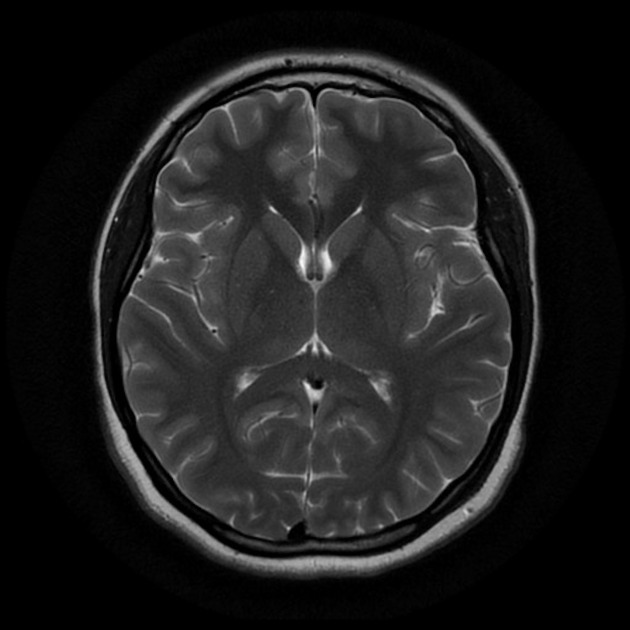
\includegraphics[height=0.2\textheight]{intro/cancerno.png}
     \caption{Healthy brain}
     \label{fig:cancerno}
  \end{subfigure}
  \hfill
  \begin{subfigure}{0.49\textwidth}
     \centering
     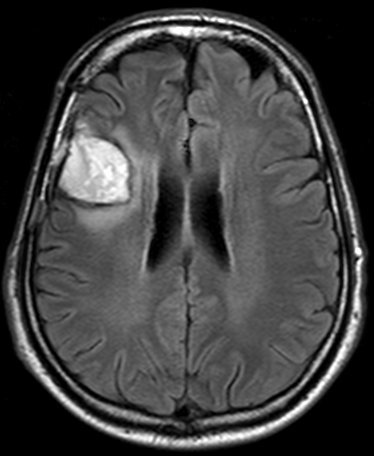
\includegraphics[height=0.2\textheight]{intro/canceryes.png}
     \caption{Brain with a tumor}
     \label{fig:canceryes}
  \end{subfigure}
  \caption[Healthy brain with tumor brain comparison]{Comparison of two magnetic resonance images of the brain. The brain on the left is healthy, whereas the brain on the right has a clearly visible tumor at the top left. These images are coming from the Kaggle brain dataset~\cite{noauthor_brain_nodate}.}
  \label{fig:canceryesno}
\end{figure}


\section{Motivation}
As seen in the previous section, cancer is very dangerous and leads to a significant amount of deaths per year, but mortality can be reduced by an early diagnosis, or a performant and precise screening. This work has been done to ensure a better performance of early diagnoses. Since 2018, the cantonal hospital of Fribourg \mbox{(H-FR)} has been collaborating with the eXascale Infolab at the University of Fribourg (UniFR) to create and develop a CAD system that can help the radiologists in their work, to analyze and find early stages of cancer as soon as possible. This project has been called \emph{Hydra}.

Hydra has been created by using machine learning techniques, as a part of artificial intelligence. The software looks at medical images, and predicts whether there is or not a tumor in the image. In that way, radiologists can be warned earlier to start the treatment of a cancer, which will hopefully result in saving lives. To train such a method, a huge amount of data is needed. Worldwide medical institutions have given public access to their anonymized data. Researchers can then use this data to do similar work as the presented one.

This work is a part of the full Hydra framework. The project has been started with the two past works of \citet{clement_prostate_2020, lee_p-hydra_2020}, who first created the machine learning model that will be used to detect and locate possible tumor in a medical image. They have use three different medical datasets, and try different methods to train the software in an optimal manner. These three datasets are the PROSTATEx~\cite{armato_prostatex_2018} dataset, the Lung CT Challenge~\cite{kirby_lungx_2016} dataset and the Kaggle brain~\cite{noauthor_brain_nodate} dataset.

This thesis will present first in Chapter~\ref{ch:mlbasics} some machine learning concepts and backgrounds that has to be known before getting in the project. It includes a small introduction on machine learning, and how to construct mathematical models that will be train on the data, with some powerful techniques such as neural networks. In Chapter~\ref{ch:datasets}, an introduction about the types of medical images will be made. The way these images are handle by a computer will also be shown. Then, the three new datasets will be presented. Their content as well as their origin will be explained. In Chapter~\ref{ch:preprocscripts}, the contributions (see Section~\ref{sec:contributions}) of this work will be developed. Finally, a conclusion about this work and the future work that has to be done can be found in Chapter~\ref{ch:conclusion}.

\section{Contributions}
\label{sec:contributions}
To improve the Hydra framework, this work will add three more datasets that will be used. These datasets are also publicly available. The more data is used, the more Hydra will be performant. Before using this data, it has to be preprocessed first. Indeed, the software can not read directly the raw medical images, but they have to be modified so that they can be readable by the software.

The main contributions of this work, in the continuation of the Hydra project, are then:

\vbox{
  \begin{itemize}
    \item A new module that creates segmentation masks from tumor contours
    \item Three new preprocessing scripts that will preprocess the three new datasets
    \item Minor improvements on the past work
  \end{itemize}}

The Hydra framework is written in the Python programming language, that is a well used and referenced language for machine learning projects. The full code of the contributions made in this work is publicly available on GitHub\footnote{\url{https://github.com/ChristopheBroillet/Hydra_Segmentation}}.
